
\begin{figure}
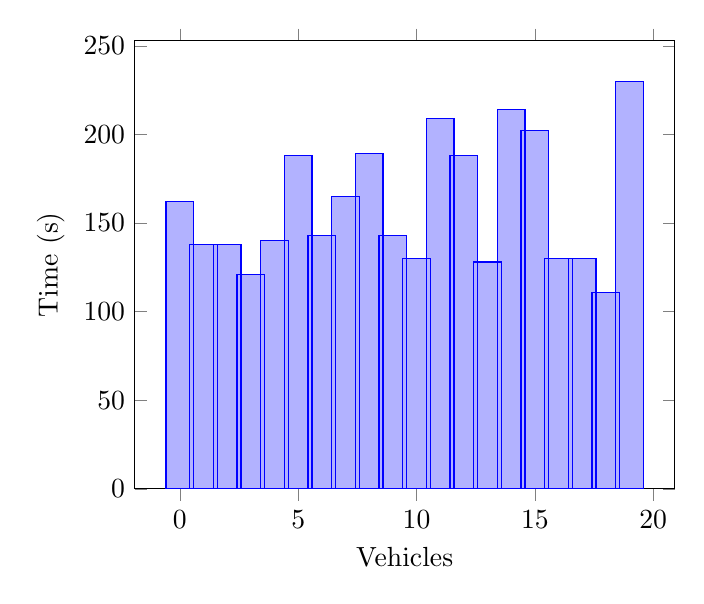
\begin{tikzpicture}
\begin{axis}[
legend style={anchor=west},
xlabel=Vehicles,
ylabel=Time (s),
ymin=0,
ybar,
]
\addplot coordinates {
(0, 162)
(1, 138)
(2, 138)
(3, 121)
(4, 140)
(5, 188)
(6, 143)
(7, 165)
(8, 189)
(9, 143)
(10, 130)
(11, 209)
(12, 188)
(13, 128)
(14, 214)
(15, 202)
(16, 130)
(17, 130)
(18, 111)
(19, 230)
};

\end{axis}
\end{tikzpicture}
\label{tik:0:18_N, 18_N.-60, 17_N, 15_S, 15_S.-30, 13_N, 13_N.-40, 11_N, 8_N, 7_N, 7_N.-60, 5_N, 4_N, 4_N.-60, 2_V}
\caption{0 percent diving with GSC on route $18_N, 18_N.-60, 17_N, 15_S, 15_S.-30, 13_N, 13_N.-40, 11_N, 8_N, 7_N, 7_N.-60, 5_N, 4_N, 4_N.-60, 2_V$}
\end{figure}
